% Drawing 154/09-5 -- folder 154, batch 09, archive page 167 (PDF page 168).
% Transcription: dessins en couleur sans texte suivi : plusieurs disques bordés de vert clair ou de vert foncé traversés de pseudo-droites rouges, certains secteurs coloriés en jaune, des sommets marqués d'un point ; des faisceaux de pseudo-droites rouges qui enjambent une droite vert clair en arc, ou se referment en fuseaux au-dessus et au-dessous d'un segment vert foncé ; dans l'un de ces fuseaux, les marques $D$, $D'$, $D''$ et une suite de petits $0$ et $1$ le long des droites ; une bande de fuseaux rouges séparés par des traits vert clair, avec de petits $0$ ; en bas à droite, en noir, une grille de droites dont une vert clair
% Kind: disks with arrangements and yellow sectors; pencils of pseudolines straddling a line; cylinders and bands; grid. Method 2 (schematic redraw from the facsimile). Status: partial.
% Notes: Colour drawings without running text, read from the page view: several disks bordered in light or dark green crossed by red pseudolines, some sectors coloured yellow (drawn as wedges), vertices marked with a point; pencils of red pseudolines straddling a light green line (a half-disk on a line, a cylinder on a line, an oval with stacked arcs on a line, labelled D, D', D'' as far as legible); two lines cut by orange lines; small cylinders and a band of red spindles round a dark green line; a small grid of black and light green lines. Strands schematic.
% Coordinates: 1 unit = 1 mm = 1/100 of the crop width (bbox in page fractions: [0.121, 0.121, 0.918, 0.47]).
% Redrawn by Claude (claude-opus-5-5), issue #73, 2026-11-07; not checked by a human; not compiled (no TeX in the session).
% Rights: reproduces part of the work -- behind RENDER_TRANSCRIPTS, never published by itself.
\documentclass[tikz,border=3pt]{standalone}
\usepackage{amsmath,amssymb}
\usetikzlibrary{patterns,arrows.meta}
\tikzset{Or/.style={orange!90!black}, Ye/.style={yellow!80!orange}, Lg/.style={green!60!black!70}, Dg/.style={green!45!black}, Br/.style={brown!80!black}, Rd/.style={red!85!black}, Bl/.style={blue!70!black}, Gy/.style={black!40}, pencil/.style={black!45}, struck/.style={black!35}, mark/.style={circle,draw,inner sep=1.3pt}, pt/.style={circle,fill,inner sep=0.9pt}, opt/.style={circle,draw,fill=white,inner sep=1.1pt}}
\begin{document}
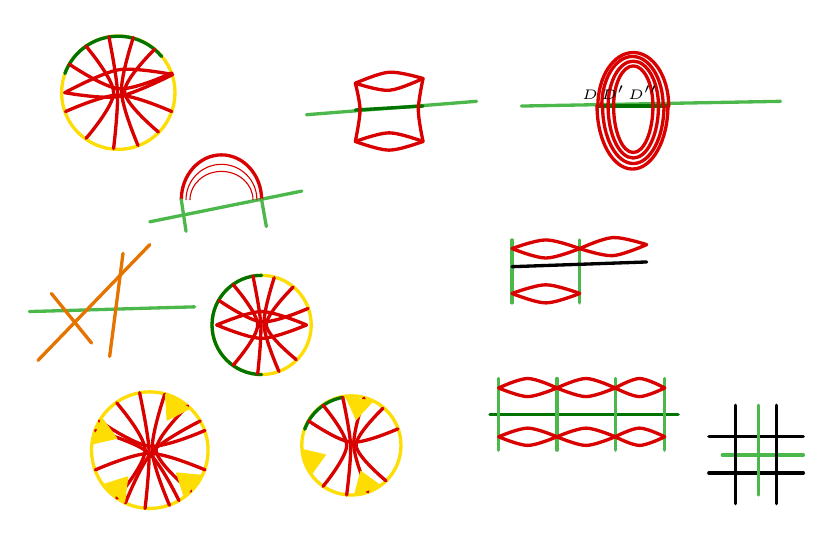
\begin{tikzpicture}[x=1mm,y=1mm,line cap=round,line join=round,font=\scriptsize]
\draw[Ye,very thick] (11.9,-8) circle[radius=7.2];
\draw[Dg,very thick] (17.4,-3.4) arc[start angle=40, end angle=160, x radius=7.2, y radius=7.2];
\draw[Rd,very thick] plot[smooth, tension=0.55] coordinates {(10.7,-0.9) (11.8,-8) (11.3,-15.1)};
\draw[Rd,very thick] plot[smooth, tension=0.55] coordinates {(13.8,-1) (12.3,-7.9) (14.4,-14.7)};
\draw[Rd,very thick] plot[smooth, tension=0.55] coordinates {(7.8,-2.1) (11.3,-8) (7.8,-13.8)};
\draw[Rd,very thick] plot[smooth, tension=0.55] coordinates {(16.5,-2.5) (12.7,-7.9) (17,-13)};
\draw[Rd,very thick] plot[smooth, tension=0.55] coordinates {(5.7,-4.4) (12,-7.5) (18.7,-5.5)};
\draw[Rd,very thick] plot[smooth, tension=0.55] coordinates {(5.2,-10.4) (11.9,-8.3) (18.7,-10.4)};
\draw[Rd,very thick] plot[smooth, tension=0.55] coordinates {(5.1,-8) (11.9,-5.1) (18.8,-5.7)};
\draw[Rd,very thick] plot[smooth, tension=0.55] coordinates {(5.1,-8) (11.9,-8.5) (18.8,-5.7)};
\draw[Lg,very thick] (15.9,-24.4) -- (35.2,-20.5);
\draw[Rd,very thick] (30.1,-21.6) arc[start angle=0, end angle=180, x radius=5.1, y radius=5.7];
\draw[Rd] (29.5,-21.6) arc[start angle=0, end angle=180, x radius=4.5, y radius=4.5];
\draw[Rd] (29,-21.6) arc[start angle=0, end angle=180, x radius=4, y radius=3.6];
\draw[Lg,very thick] (19.9,-21.6) -- (20.5,-25.6);
\draw[Lg,very thick] (30.1,-21.6) -- (30.7,-25);
\draw[Lg,very thick] (35.8,-10.8) -- (57.4,-9.1);
\draw[Dg,very thick] (42,-10.2) -- (50.6,-9.7);
\draw[Rd,very thick] plot[smooth, tension=0.55] coordinates {(42,-6.8) (46.3,-5.4) (50.6,-6.2)};
\draw[Rd,very thick] plot[smooth, tension=0.55] coordinates {(42,-6.8) (46.3,-7.7) (50.6,-6.2)};
\draw[Rd,very thick] plot[smooth, tension=0.55] coordinates {(42,-14.2) (46.3,-13.1) (50.6,-14.2)};
\draw[Rd,very thick] plot[smooth, tension=0.55] coordinates {(42,-14.2) (46.3,-15.3) (50.6,-14.2)};
\draw[Rd,very thick] plot[smooth, tension=0.55] coordinates {(42,-6.8) (42.6,-10.2) (42,-14.2)};
\draw[Rd,very thick] plot[smooth, tension=0.55] coordinates {(50.6,-6.2) (50,-10.2) (50.6,-14.2)};
\draw[Lg,very thick] (63.1,-9.7) -- (96,-9.1);
\draw[Dg,very thick] (72.7,-9.7) -- (81.8,-9.7);
\draw[Rd,very thick] (81.8,-9.7) arc[start angle=0, end angle=180, x radius=4.5, y radius=6.8];
\draw[Rd,very thick] (81.1,-9.7) arc[start angle=0, end angle=180, x radius=3.9, y radius=6.3];
\draw[Rd,very thick] (80.5,-9.7) arc[start angle=0, end angle=180, x radius=3.2, y radius=5.7];
\draw[Rd,very thick] (79.8,-9.7) arc[start angle=0, end angle=180, x radius=2.5, y radius=5.1];
\draw[Rd,very thick] (72.7,-9.7) arc[start angle=180, end angle=360, x radius=4.5, y radius=8];
\draw[Rd,very thick] (73.4,-9.7) arc[start angle=180, end angle=360, x radius=3.9, y radius=7.3];
\draw[Rd,very thick] (74.1,-9.7) arc[start angle=180, end angle=360, x radius=3.2, y radius=6.6];
\draw[Rd,very thick] (74.8,-9.7) arc[start angle=180, end angle=360, x radius=2.5, y radius=5.9];
\node[inner sep=1pt] at (75.6,-8) {\tiny $D\,D'\,D''$};
\draw[Lg,very thick] (0.6,-35.8) -- (21.6,-35.2);
\draw[Or,very thick] (1.7,-42) -- (15.9,-27.3);
\draw[Or,very thick] (3.4,-33.5) -- (8.5,-39.8);
\draw[Or,very thick] (12.5,-28.4) -- (10.8,-41.5);
\draw[Ye,very thick] (30.1,-37.5) circle[radius=6.3];
\draw[Dg,very thick] (30.1,-31.2) arc[start angle=90, end angle=270, x radius=6.3, y radius=6.3];
\draw[Rd,very thick] plot[smooth, tension=0.55] coordinates {(24.4,-37.5) (30.1,-35.8) (35.8,-37.5)};
\draw[Rd,very thick] plot[smooth, tension=0.55] coordinates {(24.4,-37.5) (30.1,-39.2) (35.8,-37.5)};
\draw[Rd,very thick] plot[smooth, tension=0.55] coordinates {(29,-31.3) (30,-37.5) (29.6,-43.7)};
\draw[Rd,very thick] plot[smooth, tension=0.55] coordinates {(31.7,-31.5) (30.4,-37.5) (32.3,-43.4)};
\draw[Rd,very thick] plot[smooth, tension=0.55] coordinates {(26.5,-32.4) (29.6,-37.5) (26.5,-42.6)};
\draw[Rd,very thick] plot[smooth, tension=0.55] coordinates {(34.1,-32.7) (30.7,-37.5) (34.5,-41.9)};
\draw[Rd,very thick] plot[smooth, tension=0.55] coordinates {(24.7,-34.4) (30.1,-37.1) (36,-35.4)};
\draw[Ye,very thick] (15.9,-53.4) circle[radius=7.4];
\draw[Rd,very thick] plot[smooth, tension=0.55] coordinates {(14.6,-46.1) (15.8,-53.4) (15.3,-60.8)};
\draw[Rd,very thick] plot[smooth, tension=0.55] coordinates {(17.8,-46.3) (16.2,-53.4) (18.4,-60.4)};
\draw[Rd,very thick] plot[smooth, tension=0.55] coordinates {(11.7,-47.4) (15.3,-53.4) (11.7,-59.5)};
\draw[Rd,very thick] plot[smooth, tension=0.55] coordinates {(20.7,-47.8) (16.7,-53.4) (21.1,-58.6)};
\draw[Rd,very thick] plot[smooth, tension=0.55] coordinates {(9.5,-49.7) (15.9,-52.9) (22.9,-50.9)};
\draw[Rd,very thick] plot[smooth, tension=0.55] coordinates {(9,-55.9) (15.9,-53.8) (22.9,-55.9)};
\draw[Rd,very thick] plot[smooth, tension=0.55] coordinates {(22.3,-49.7) (16.2,-53.6) (12.8,-60.1)};
\draw[Rd,very thick] plot[smooth, tension=0.55] coordinates {(9,-50.9) (15.7,-53.7) (19.6,-59.8)};
\draw[Ye] (21,-48.1) -- (17.9,-46.3) -- (18.1,-49.6) -- cycle;
\fill[pattern=north east lines,Ye] (21,-48.1) -- (17.9,-46.3) -- (18.1,-49.6) -- cycle;
\draw[Ye] (9.8,-49.3) -- (8.6,-52.6) -- (11.7,-51.9) -- cycle;
\fill[pattern=north east lines,Ye] (9.8,-49.3) -- (8.6,-52.6) -- (11.7,-51.9) -- cycle;
\draw[Ye] (9.9,-57.8) -- (12.7,-60) -- (13.1,-56.8) -- cycle;
\fill[pattern=north east lines,Ye] (9.9,-57.8) -- (12.7,-60) -- (13.1,-56.8) -- cycle;
\draw[Ye] (20.3,-59.4) -- (22.5,-56.6) -- (19.3,-56.3) -- cycle;
\fill[pattern=north east lines,Ye] (20.3,-59.4) -- (22.5,-56.6) -- (19.3,-56.3) -- cycle;
\draw[Ye,very thick] (41.5,-52.8) circle[radius=6.3];
\draw[Dg,very thick] (40.4,-46.7) arc[start angle=100, end angle=160, x radius=6.3, y radius=6.3];
\draw[Rd,very thick] plot[smooth, tension=0.55] coordinates {(40.4,-46.7) (41.4,-52.8) (40.9,-59.1)};
\draw[Rd,very thick] plot[smooth, tension=0.55] coordinates {(43.1,-46.8) (41.8,-52.8) (43.6,-58.7)};
\draw[Rd,very thick] plot[smooth, tension=0.55] coordinates {(37.9,-47.7) (40.9,-52.8) (37.9,-58)};
\draw[Rd,very thick] plot[smooth, tension=0.55] coordinates {(45.5,-48.1) (42.1,-52.8) (45.9,-57.3)};
\draw[Rd,very thick] plot[smooth, tension=0.55] coordinates {(36.1,-49.7) (41.5,-52.4) (47.4,-50.7)};
\draw[Ye] (44.2,-47.2) -- (40.8,-46.6) -- (42.1,-49.5) -- cycle;
\fill[pattern=north east lines,Ye] (44.2,-47.2) -- (40.8,-46.6) -- (42.1,-49.5) -- cycle;
\draw[Ye] (35.2,-53.3) -- (36.4,-56.5) -- (38.2,-54) -- cycle;
\fill[pattern=north east lines,Ye] (35.2,-53.3) -- (36.4,-56.5) -- (38.2,-54) -- cycle;
\draw[Ye] (41.9,-59.1) -- (45.2,-57.9) -- (42.7,-56.1) -- cycle;
\fill[pattern=north east lines,Ye] (41.9,-59.1) -- (45.2,-57.9) -- (42.7,-56.1) -- cycle;
\draw[Lg,very thick] (61.9,-26.7) -- (61.9,-34.7);
\draw[Lg,very thick] (70.5,-26.7) -- (70.5,-34.7);
\draw[Rd,very thick] plot[smooth, tension=0.55] coordinates {(61.9,-27.8) (66.2,-26.7) (70.5,-27.8)};
\draw[Rd,very thick] plot[smooth, tension=0.55] coordinates {(61.9,-27.8) (66.2,-29) (70.5,-27.8)};
\draw[Rd,very thick] plot[smooth, tension=0.55] coordinates {(61.9,-33.5) (66.2,-32.4) (70.5,-33.5)};
\draw[Rd,very thick] plot[smooth, tension=0.55] coordinates {(61.9,-33.5) (66.2,-34.7) (70.5,-33.5)};
\draw[Rd,very thick] plot[smooth, tension=0.55] coordinates {(70.5,-27.8) (74.7,-26.4) (79,-27.3)};
\draw[Rd,very thick] plot[smooth, tension=0.55] coordinates {(70.5,-27.8) (74.7,-28.7) (79,-27.3)};
\draw[very thick] (61.9,-30.1) -- (79,-29.5);
\draw[Dg,very thick] (59.1,-48.9) -- (83,-48.9);
\draw[Lg,very thick] (60.2,-44.3) -- (60.2,-53.4);
\draw[Lg,very thick] (67.6,-44.3) -- (67.6,-53.4);
\draw[Lg,very thick] (75,-44.3) -- (75,-53.4);
\draw[Lg,very thick] (81.3,-44.3) -- (81.3,-53.4);
\draw[Rd,very thick] plot[smooth, tension=0.55] coordinates {(60.2,-45.5) (63.9,-44.3) (67.6,-45.5)};
\draw[Rd,very thick] plot[smooth, tension=0.55] coordinates {(60.2,-45.5) (63.9,-46.6) (67.6,-45.5)};
\draw[Rd,very thick] plot[smooth, tension=0.55] coordinates {(67.6,-45.5) (71.3,-44.3) (75,-45.5)};
\draw[Rd,very thick] plot[smooth, tension=0.55] coordinates {(67.6,-45.5) (71.3,-46.6) (75,-45.5)};
\draw[Rd,very thick] plot[smooth, tension=0.55] coordinates {(75,-45.5) (78.1,-44.3) (81.3,-45.5)};
\draw[Rd,very thick] plot[smooth, tension=0.55] coordinates {(75,-45.5) (78.1,-46.6) (81.3,-45.5)};
\draw[Rd,very thick] plot[smooth, tension=0.55] coordinates {(60.2,-51.7) (63.9,-50.6) (67.6,-51.7)};
\draw[Rd,very thick] plot[smooth, tension=0.55] coordinates {(60.2,-51.7) (63.9,-52.8) (67.6,-51.7)};
\draw[Rd,very thick] plot[smooth, tension=0.55] coordinates {(67.6,-51.7) (71.3,-50.6) (75,-51.7)};
\draw[Rd,very thick] plot[smooth, tension=0.55] coordinates {(67.6,-51.7) (71.3,-52.8) (75,-51.7)};
\draw[Rd,very thick] plot[smooth, tension=0.55] coordinates {(75,-51.7) (78.1,-50.6) (81.3,-51.7)};
\draw[Rd,very thick] plot[smooth, tension=0.55] coordinates {(75,-51.7) (78.1,-52.8) (81.3,-51.7)};
\draw[very thick] (86.9,-51.7) -- (98.9,-51.7);
\draw[very thick] (86.9,-56.3) -- (98.9,-56.3);
\draw[Lg,very thick] (88.6,-54) -- (98.9,-54);
\draw[very thick] (90.3,-47.7) -- (90.3,-60.2);
\draw[very thick] (95.5,-47.7) -- (95.5,-60.2);
\draw[Lg,very thick] (93.2,-47.7) -- (93.2,-59.1);
\end{tikzpicture}
\end{document}
